

\section{Dataset and Study Area}
\label{sec:stage4}

 Two datasets are primarily used in this study.  A subset (image sub-fragment) of the UAVSAR L-band SAR dataset has been used to study the experiment parameters and actions. The classification is carried out on larger a ALOS-2 L-band SAR image with extensive performance analysis.
 
 
\subsubsection{Dataset Description: UAVSAR L-Band dataset}

The first dataset is a Single Look Complex L-Band UAVSAR dataset acquired over the San Francisco bay area, USA on November 13, 2012, with a resolution of $\SI{0.6}{\m}$ in azimuth and $\SI{1.6}{\m}$ in range. The look angle ranges from $25^\circ$ to $60^\circ$ with a range swath of $\SI{20}{\km}$~\cite{fore2015uavsar}.   This is an air-borne sensor capable of acquiring very high resolution images. The data are multi-looked 3 times in range and 12 times in azimuth to bring them to a resolution of $\SI{7.2}{\m}$ in azimuth and $\SI{5}{\m}$ in range to make them comparable in spatial resolution to the space-borne ALOS-2 dataset. A $1000\times1000$ pixel representative portion is used for these experiments. This data-set is freely available and has similar properties to the space-borne ALOS-2 sensor, so it was used to analyze the action of the network. The subset has a prominent urban area rotated with respect to the radar line of sight, which was used to check the effectiveness of the technique. 

\subsubsection{Dataset Description: ALOS-2 L-Band dataset}
The second dataset is an ALOS-2 image acquired on March 24, 2015 over the city of San Francisco, USA with a resolution of $\SI{3.2}{\m}$ in range and $\SI{2.8}{\m}$ in azimuth. The dataset is multi-looked 3 times in range and 2 times in azimuth to generate an image of resolution $\SI{9.6}{\m}$ in range and $\SI{5.6}{\m}$ in azimuth. The radar operates in L-Band with $\lambda=\SI{24}{\cm}$. The area is heavily urbanized and has high coverage with airborne and space-borne polarimetric radar creating a sizable well documented data-pool that can be exploited for various deep learning techniques. Consequently, this area has been featured in several studies on PolSAR~\cite{lee2004classification, bhattacharya2015adaptive}.

\begin{figure}[htbp]
	\centering
	\begin{subfigure}[t]{0.6\columnwidth}
	\centering
	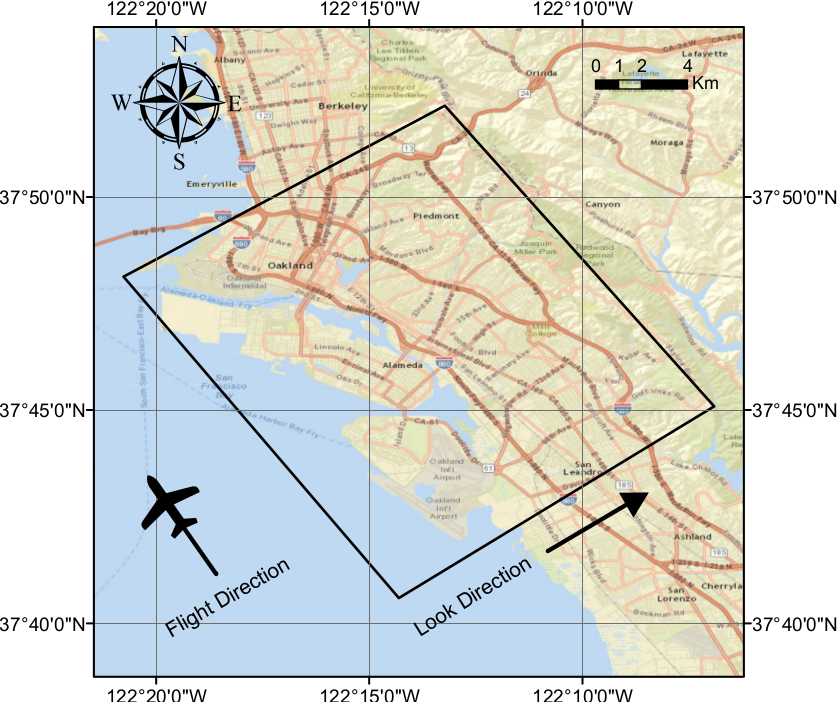
\includegraphics[width =\columnwidth]{Figures/Map} \quad
	%\caption{$\alpha_0$}
	\vspace{-10pt}
	\caption{}
	%\label{fig:alpha}
 	\end{subfigure}%
% 	 ~ 

\vspace{5pt}

	\begin{subfigure}[t]{0.4\columnwidth}
	\centering
	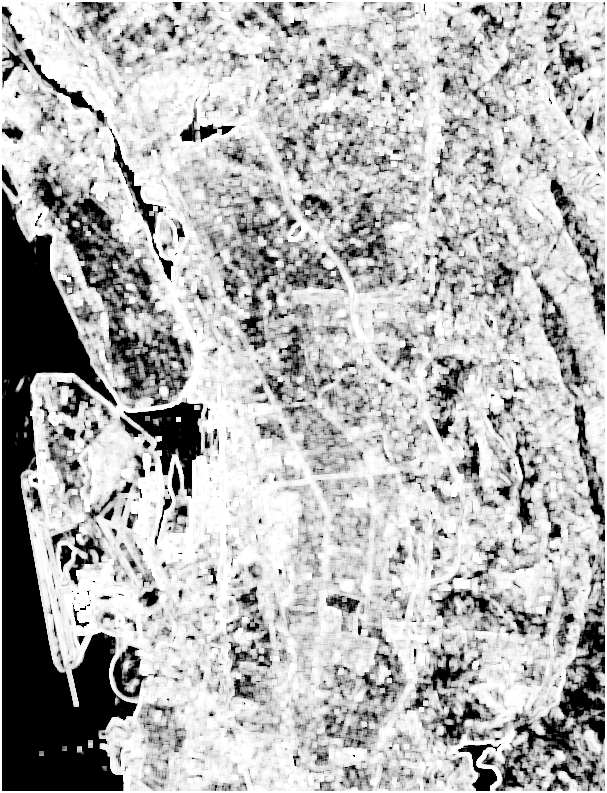
\includegraphics[width = \columnwidth]{Figures/IGRASS15_WORK/alpha_5_5}
	%\caption{$\alpha_0$}
	\caption{}
	%\label{fig:alpha}
	 \end{subfigure}%
	    ~ 
	 \begin{subfigure}[t]{0.4\columnwidth}
	 \centering
	 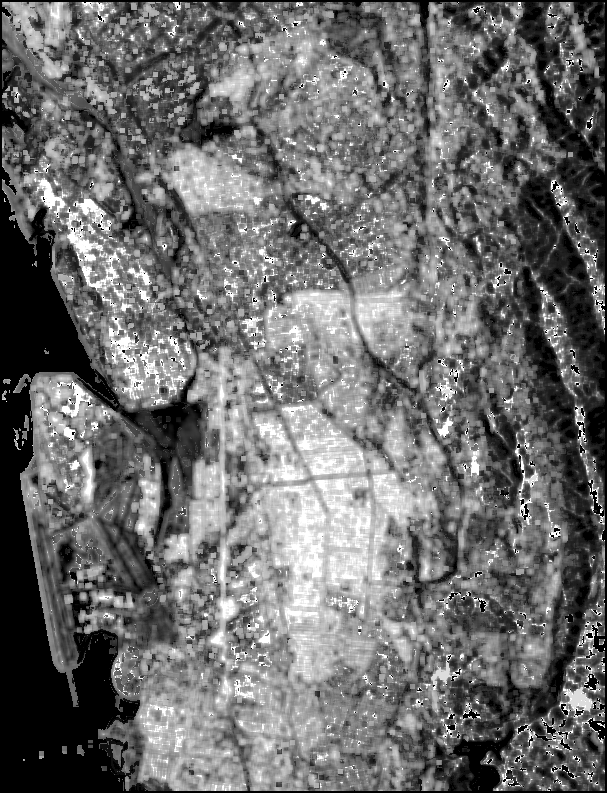
\includegraphics[width = \columnwidth]{Figures/IGRASS15_WORK/gamma_5_5}
	 %\caption{$\gamma_0$}
 	\caption{}
	 %	\caption[PolSAR data preprocessing]{Orientation.}
	 %	\label{fig:gamma}
	 \end{subfigure}   
	 \caption{(a) A map with the dataset footprint shown with the (b) $\alpha^0$ and (c) $\gamma^0$ images extracted from a UAVSAR L-Band dataset collected over Oakland. These serve as textural information to the classifier.}
	 \label{fig:alphagamma}
\end{figure}


By operating in L-Band, ALOS-2 has increased penetration capability and is less susceptible to scattering due to surface roughness. As a result, return from areas of smooth vegetation such as parks and golf courses appear to have undergone specular reflection, and consequently have very low return power levels. The average backscattered power  in these areas for the co-polarized channels, $\sigma^0_{hh} \approx -16\mathrm{dB}$,  and $\sigma^0_{vv} \approx -15\mathrm{dB}$. This is comparable to that of still water, which is about $\sigma^0_{hh} \approx \sigma^0_{vv} \approx -19\mathrm{dB}$ and is much lower than the power returned from forest areas, where $\sigma^0_{hh} \approx 6\mathrm{dB}$ and $\sigma^0_{vv} \approx 7\mathrm{dB}$. Consequently the areas having very low backscatter power tend to be classified as belonging to the water class. This phenomenon is a function of the incidence angle of the sensor and the relative roughness of the surface  with respect to the sensing wavelength. 




\begin{figure}
\centering
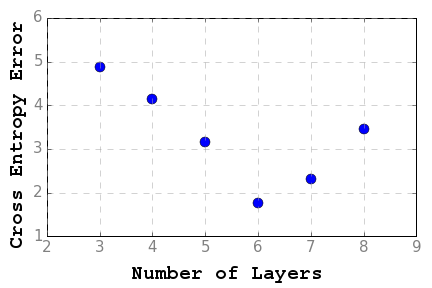
\includegraphics[width=0.6\columnwidth]{Figures/layers}
\caption{Effect of layer depth on training of AE in terms of cross entropy error versus the number of layers.}
\label{fig:layerplot}
\end{figure}




\section{Experimental Set-Up}
\label{sec:expt_cathay312}

`Urban', `Forest/vegetation' and `Water' are the classes chosen in this study. These   classes are usually an important input for various applications related to urban classification. Disaster management studies, urban sprawl estimation, target and infrastructure recognition are examples of applications that benefit from accurate identification of these classes. The urban class comprises of man-made structures which height is equal to or greater than  the sensing wavelength causing the incident EM wave to undergo even number of bounces from the surface surrounding the structure, and  the structure itself before returning back to the sensor. This includes structures like houses, walls, masts etc. These targets are characterized in PolSAR data by a strong double bounce return because of their constituent materials and geometry~\cite{elachi1990radar}.
%In many instances, the challenge in the classification of such a structures is their orientation about the radar line of sight and range or azimuth slopes. In this condition the polarized return, $hh$ and $vv$, is deflected away from the sensor, while a high cross polarized echo is returned. This is generally expected from natural areas such as vegetation causing misclassification.
%The deflection of the polarized return away, and cross polarized echo towards the sensor from urban areas oriented away from the radar line of sight causes it to be confused with natural areas such as vegetation causing misclassification.
In the context of this study, the `Forest / Vegetation' class is used to refer to areas of natural vegetation, open spaces between urban areas with light to almost no vegetation, parks etc. In PolSAR, this class is characterized  by diffused scattering which does not change significantly with rotation about the radar line of sight. The `Water' class is made up of water bodies that are characterized by specular or surface reflection depending on the condition of the surface. At longer wavelengths, some smooth natural areas have a very low return and tends to be misclassified as water. The proportion of such pixels is however under 0.2\% of the total as estimated from the ground truth. 



% SAR preprocessing
As a part of the SAR pre-processing, a refined Lee Filter with a window size of $3\times3$ is applied to the dataset after the application of appropriate multi-looking for the suppression of speckle. The areas under consideration have relatively flat topography, and hence no radiometric terrain correction is applied. Appropriate compensation~\cite{atwood2012improving} may be applied in case of highly undulated areas. 
The synthetic target database is generated by rotating $\mathbf{T}$ with a step size of $3^\circ$ in the range  $-22^\circ$  to $22^\circ$. Considering a finer sampling of $1^\circ$ increases the data volume many-fold without a corresponding appreciable increase in classification accuracy.

The network used in stage 2 of the proposed method is a six layer stacked sparse auto-encoder. To determine the optimal number of layers the dataset was trained on different AE topologies of increasing depth, but with the same hyper-parameters ($\alpha=0.01,\Gamma=0.1,\mu=0.95$). The cross-entropy error at the end of training was analyzed to compare the architectures. From the plot in Figure~\ref{fig:layerplot} it is seen that a 6-layer auto-encoder is the most suitable for this dataset. From input $X$ to output $X'$, the network has $1024,\ 512,\ 256$ nodes in layers 1, 2 and 3, respectively, forming the encoder, and $512,\ 1024$ nodes in layer 5 and 6 forming the decoder. The central $64$ node layer 4 contains the learned representation. The non-linearity of each encoder is a ReLU with a leakage parameter $\alpha_r = 0.01$ allowing the handling of large dynamic range input without saturating or becoming non-responsive over many iterations. The sparsity hyper-parameter of the network is set to $\rho = 0.15$ which ensures that the average activation of each hidden neuron  is approximately near 0. %This is achieved with the addition of a penalty term to the objective function. 
The network weights and biases are randomly initialized at the beginning of each iteration using the `Xavier' strategy~\cite{glorot2010understanding}.
The network is iterated $200,000$ times with a batch size of $1000$. This ensures that the complete data set is passed multiple times though the auto-encoder for better generalization. To ensure that the learning machine is not memorizing the order in which the data are being fed, this order is randomized. The base learning rate is set to $\alpha = 0.001$ and the update step multiplier is set to $\Gamma = 0.1$. The step-size is chosen to be $40,000$ to allow for sufficient number of epochs before the learning rate is updated. The gradient descent momentum is set to $\mu = 0.85$. The value of batch size is adjusted depending on the size of the image. 

In stage 3, a three layer MLP network consisting of  $256$ hidden nodes in the first layer, $512$ in the second layer and $8$ in the last layer is used for the final classification.
When common PolSAR visualization techniques (i.e. Pauli RGB) and decompositions are applied, vegetated and rotated urban areas appear to be visually similar. This makes it more difficult to successfully discriminate and delineate rotated urban areas in a scene as compared to areas that are perpendicular to the radar line of sight.  Hence no training areas are considered from areas which do not show dihedral (red) scattering in the Pauli RGB image. 

The  weights from the representational layer of the previous stage are given as input to the MLP along with and two statistical texture parameters, $\alpha_0$ and $\gamma_0$ (Figure~\ref{fig:alphagamma}).
A window of $9\times9$ has been used for extraction of the parameters. The size of the window is determined by the resolution of the image and dimensions of the targets on the ground. These add more texture information to the classification scheme helping discern urban areas better.  For this network $\alpha=0.01$ (not to be confused with the statistical parameter $\alpha^0_{i,j}$), $\Gamma = 0.1$ and $\mu = 0.95$. About $\sim 5\%$ of the total pixels in the data-set is used for training the MLP. The MLP network is iterated a maximum of 100,000 times.


 



Five experiments are carried out on UAVSAR and ALOS-2 datasets. First, the impact of textural parameters is examined. The AE is trained and the weights of the representational layer are extracted. The MLP classification is performed both with and without the introduction of textural parameters. The difference in classification performance is evaluated in Section \ref{sec:EXPT0}. Second, the impact of the synthetic target generation is studied. The AE is trained on $\mathbf{T}$ as usual. After the completion of training the weight update is stopped and a $\mathbf{T}$ matrix rotated synthetically by $5^\circ$ and $9^\circ$ degrees is given as input. The activation pattern of the neural network in the case of permuted data is compared with the pattern when no rotation is applied (Section \ref{sec:EXPT1}).
Third, classification and performance analysis is conducted on the ALOS-2 dataset (Section \ref{sec:EXPT2}). Accuracy assessment is performed both quantitatively and qualitatively. Fourth, the response of one node of the representational layer is extracted from the AE and plotted to visualize the learned representation  (Section \ref{sec:EXPT3}). Fifth, the results of the proposed method are compared with other classification techniques (Section \ref{sec:EXPT4}).





\section{Results and Discussion}
\label{ref:results1}


The impact of textural parameters and synthetic rotation for target generation on the performance of the network are examined on a subset of the UAVSAR dataset. The analysis of classification performance using the proposed method was conducted on the full ALOS-2 scene along with the analysis of the learned representation. Finally, the performance of the proposed technique was compared with state of the art classifiers for PolSAR data. 


%The proposed technique is evaluated on a full ALOS-2 scene and compared to other polarimetric SAR classification techniques. 




\begin{figure}[tbp]
	\centering
	%	\begin{subfigure}[t]{0.35\columnwidth}
	%	\centering
	%	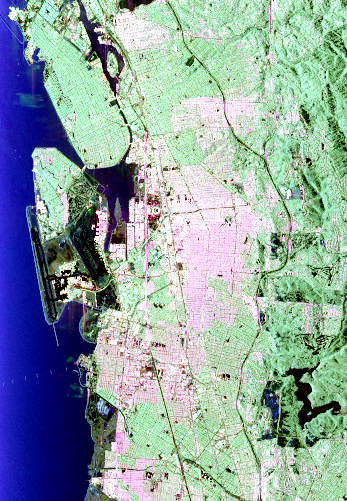
\includegraphics[width = \columnwidth]{Figures/REVIEW/PauliCrop}
	%	\caption{Pauli}
	%\label{fig:alpha}
	%	 \end{subfigure}%
	%	~    
	\begin{subfigure}[t]{0.4\columnwidth}
		\centering
		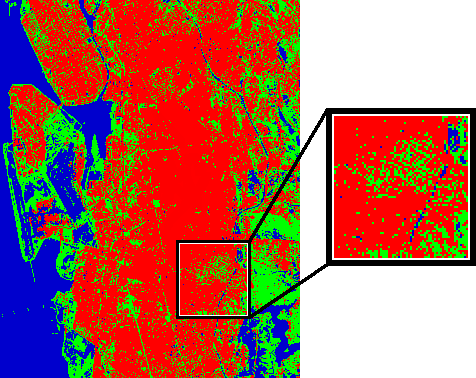
\includegraphics[width = \columnwidth]{Figures/REVIEW/TextureBZ}
		\caption{}
		%\label{fig:alpha}
	\end{subfigure}%
	~ 
	\begin{subfigure}[t]{0.4\columnwidth}
		\centering
		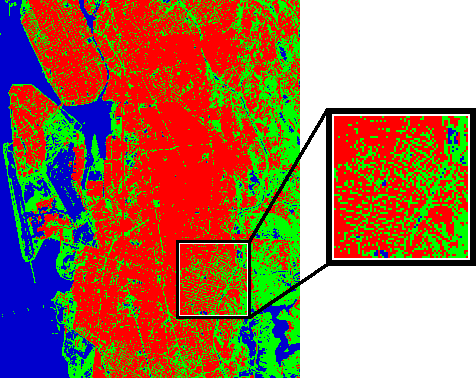
\includegraphics[width = \columnwidth]{Figures/REVIEW/NoTextureBZ}
		\caption{}
		%	\caption[PolSAR data preprocessing]{Orientation.}
		%	\label{fig:gamma}
	\end{subfigure}   
	\caption{Classified map derived from an UAVSAR full polarimetric L-Band dataset (a) with and (b) without the use of $\alpha^0$ and $\gamma^0$ as textural features. }
	\label{fig:texture}
\end{figure}

\subsubsection{Impact of Textural Parameters}
\label{sec:EXPT0}
%%% EDIT THIS
One of the advantages of the deep-learning based approach, is that useful parameters can be included in the later stages of the process. This is in contrast to approaches, where the information must be included at the beginning, causing an increase in dimensionality and classification difficulty, making a feature selection step necessary~\cite{tao2015tensorial,banerjee2014generic}.
Although the inclusion of the textural parameter only slightly improves the overall classification accuracy its inclusion can help discern low-density oriented urban targets. In Figure~\ref{fig:texture} the classification map of the UAVSAR data-set is presented, both with and without the inclusion of the textural parameters $\alpha_0$ and $\gamma_0$ in the MLP stage. The overall improvement in classification accuracy due to the inclusion of textural parameters is small ($\sim 3\%$).  However, for areas of low density sub-urban housing interleaved with vegetation and streets, an improvement is observed (black box in Figure~\ref{fig:texture}) because of benefit from the neighborhood information.  







% % % % % % % % % % % % % % % % % % % % % % 
\begin{figure} [tbp]
	\centering
	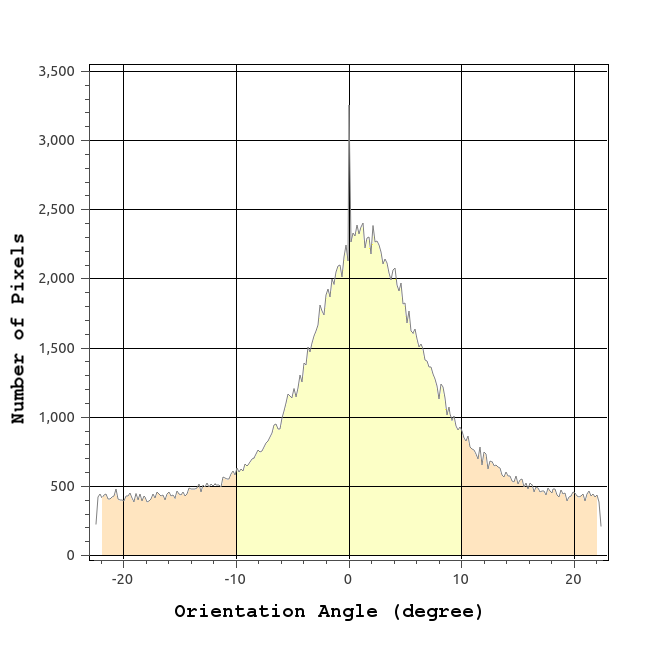
\includegraphics[width = 0.45\columnwidth]{Figures/Trento/orientation_RS2}
	\caption[PolSAR data preprocessing]{Distribution of the estimated Orientation angles of the region imaged in the UAVSAR L-Band dataset acquired over Oakland, USA.}
	\label{fig:orientationHist}
\end{figure} 
%
\begin{figure}[!htb]
	\centering
	\begin{subfigure}[t]{0.31\columnwidth}
		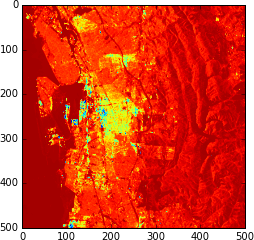
\includegraphics[width = \columnwidth]{Figures/Rotation_FS/0deg_decode3_11}
		\caption{}
		\label{fig:0deg}
	\end{subfigure}%
	~ 
	\begin{subfigure}[t]{0.31\columnwidth}
		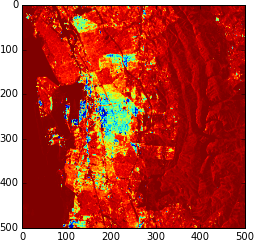
\includegraphics[width = \columnwidth]{Figures/Rotation_FS/5deg_decode3_11}
		\caption{}
		\label{fig:5deg}
	\end{subfigure}   
	~ 
	\begin{subfigure}[t]{0.31\columnwidth}
		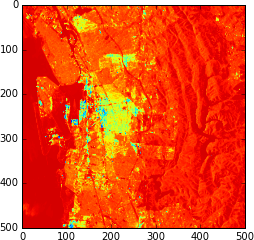
\includegraphics[width = \columnwidth]{Figures/Rotation_FS/9deg_decode3_11}
		\caption{}
		\label{fig:9deg}
	\end{subfigure}  
	
	
	%\centering
	%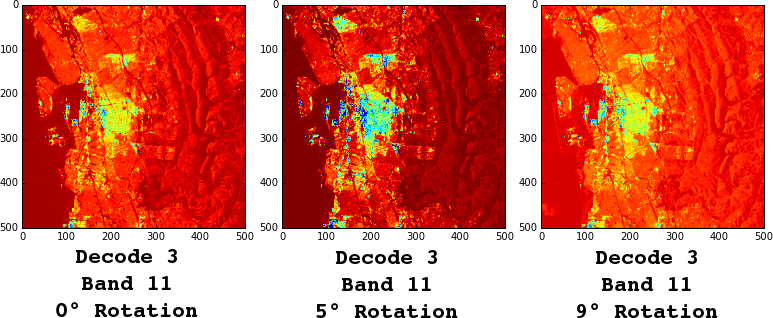
\includegraphics[width = 0.65 \columnwidth]{Figures/Rotation_FS/Rotation} \\
	% The actual value of the output of the ReLU node has been scaled from 0 to 1 for representation as an image.
	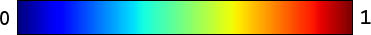
\includegraphics[width = 0.3\columnwidth]{Figures/Rotation_FS/JET}
	\caption[Effect of Rotation]{A section of the UAVSAR image is trained using the auto-encoder network and the extracted features are plotted when input corresponds to a synthetic rotation of (a)  $0^\circ$ (b) $5^\circ$  (c) $9^\circ$ respectively. The actual value of the output of the ReLU node has been scaled from 0 to 1 for representation as an image.  }
	\label{fig:rotCompare}
\end{figure} 

% % % % % % % % % % % % % % % % % % % % % % % % % % % %


\subsubsection{Impact of Synthetic Rotation}
\label{sec:EXPT1}

A histogram of measured orientation angles in the UAVSAR dataset is shown in Figure~\ref{fig:orientationHist}.  It can be seen that most of the targets are oriented between $-10^\circ$  and $10^\circ$. 
%Thus, while generating the synthetic database this range is densely subdivided as compared to the ranges $-10^\circ$  to $-22^\circ$  and $10^\circ$ to $22^\circ$. Between $-10^\circ$  and $10^\circ$ a step size of $3^\circ$ is used, while a step size of $6^\circ$ is used otherwise. 
%Considering a finer and more uniform sampling of $1^\circ$ increases the data volume many-fold without a corresponding appreciable increase in classification accuracy.
The average orientation angle of this subset is approximately $5^\circ $. The orientation angle is computed by the estimation method given in~\cite{981347}. To visualize the action of synthetic rotation, $\mathbf{T}$ is given as input to the trained AE stage after rotation by $0^\circ$, $5^\circ$ and $9^\circ$ degrees separately. As an example, the 11\textsuperscript{th} element of the feature vector is extracted, after completion of the training stage of the AE and is presented in Figure~\ref{fig:rotCompare}. In the case  of the pixels in which the synthetic rotation angle matches the actual target orientation on the ground, the reconstruction error of the AE is lower than the average one over the scene. The areas on the ground that actually correspond to the synthetic rotation ($0^\circ$, $5^\circ$ and $9^\circ$) are closer to zero. The AE was only trained on the input dataset. However it is able to provide an appropriate  response when an unseen and arbitrarily rotated version of the input data is introduced. This implies that the application of synthetic rotation to a target is equivalent to the case when such an oriented target is actually present in the training data. Thus the generalization capability of the AE is improved. 

%the areas of urban structures that were aligned by $5^\circ$ with the radar line of sight have a response closer to zero for the features extracted from the $\mathbf{\langle[T]\rangle}$ matrix which was rotated by $5^\circ$, as compared to the other input cases.   This action allows the AE to respond to a wide range of orientations, even if it is not present in the input data. This effect is exploited in the proposed technique to improve the accuracy of classification.






\begin{figure}[tbp]
\centering
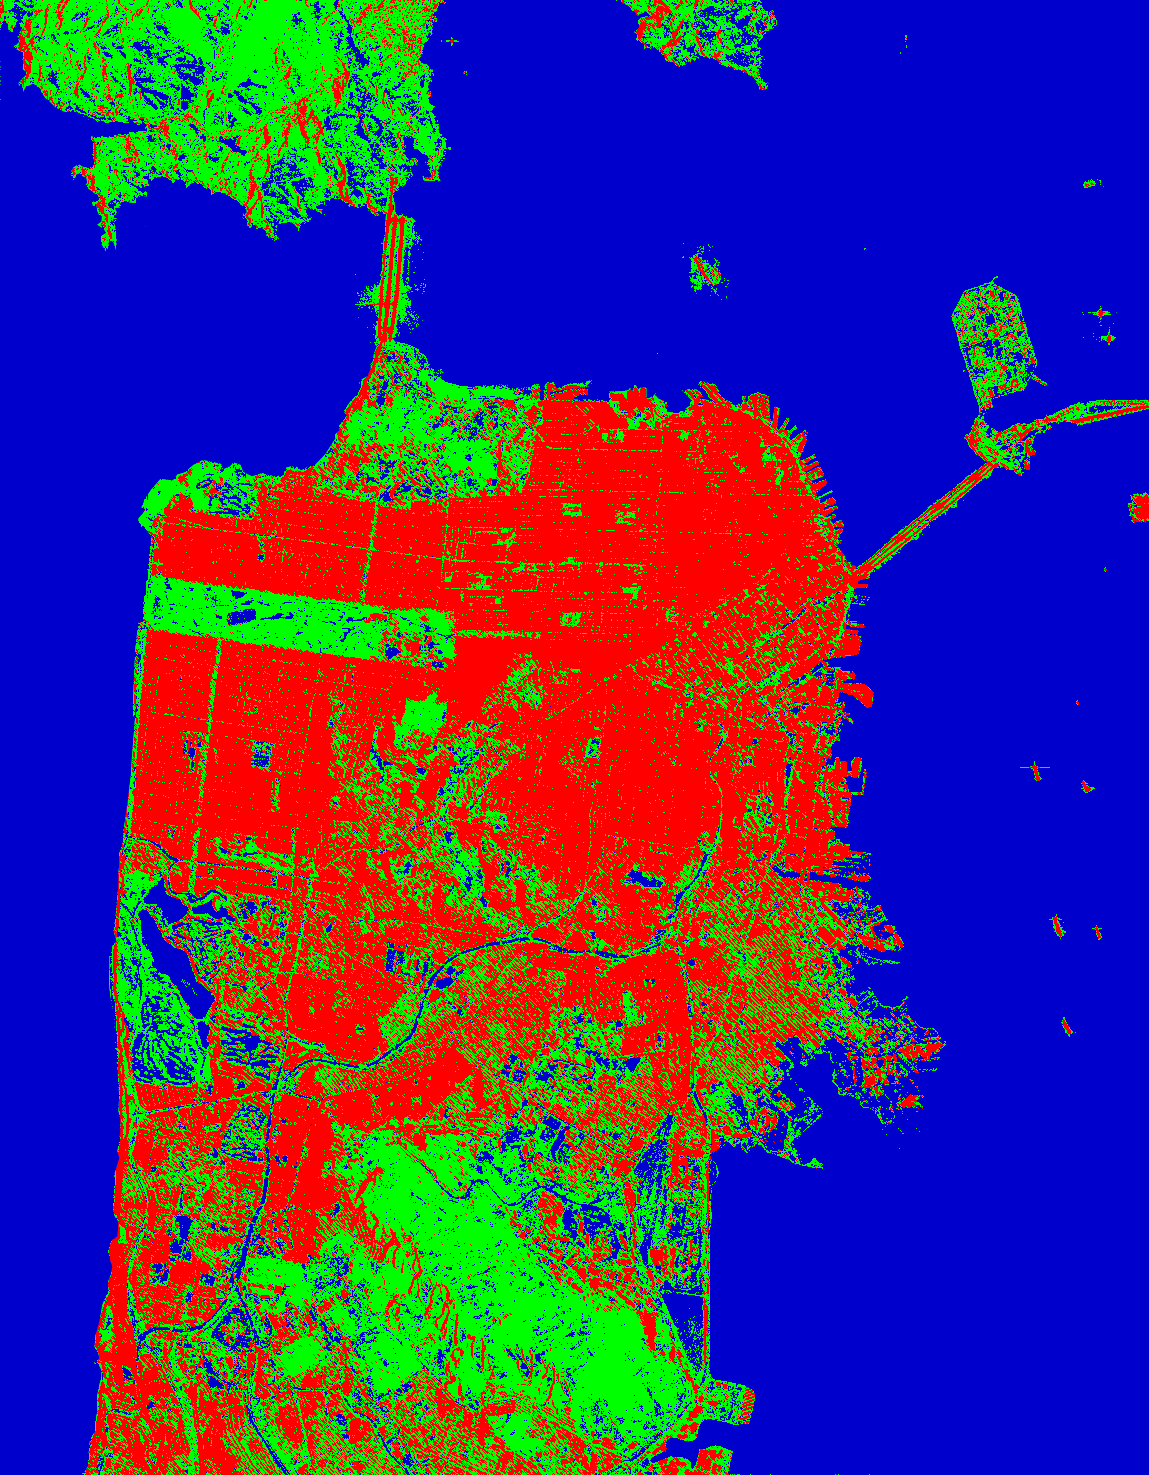
\includegraphics[width=0.5\columnwidth]{Figures/ALOS2_SF_3Class/Output_AL2_500k_alt}



		\begin{tabular}{clclcl}
					
\includegraphics[width=0.03\columnwidth]{Figures/RS2_SF_3Class/Blue.png} & Water &		
\includegraphics[width=0.03\columnwidth]{Figures/RS2_SF_3Class/Green.png} & Forest &  	
\includegraphics[width=0.03\columnwidth]{Figures/RS2_SF_3Class/Red.png} &  Urban 
		\end{tabular}
		
		\caption{Classified map of San Francisco derived from an ALOS-2 full polarimeteric L-Band dataset.}
		
\label{fig:compwal2}
\end{figure}











\begin{figure}[tbp]
\begin{subfigure}[t]{0.19\textwidth}
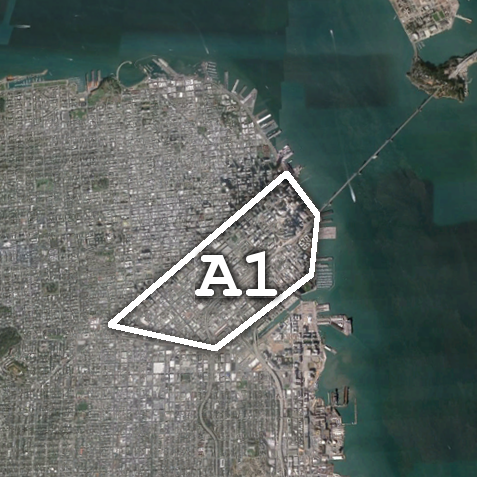
\includegraphics[width=\columnwidth]{Figures/ALOS2_SF_3Class/SouthMarketIm}  
\vspace{0.2cm}
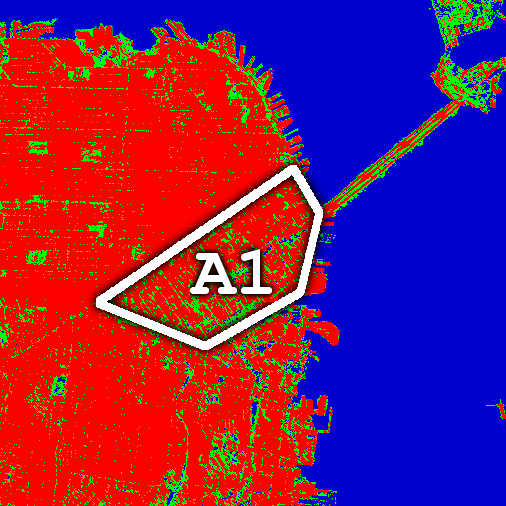
\includegraphics[width=\columnwidth]{Figures/ALOS2_SF_3Class/SouthMarket}
\caption{}
\label{fig:cla2_a}
\end{subfigure}
%\begin{subfigure}[t]{0.31\columnwidth}
%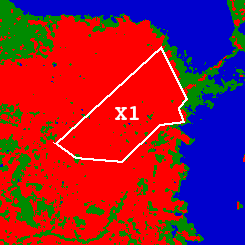
\includegraphics[width=\columnwidth]{Figures/RS2_SF_3Class/SouthOFMarket_Cl}
%\caption{South of Market}
%\end{subfigure}
\begin{subfigure}[t]{0.19\textwidth}
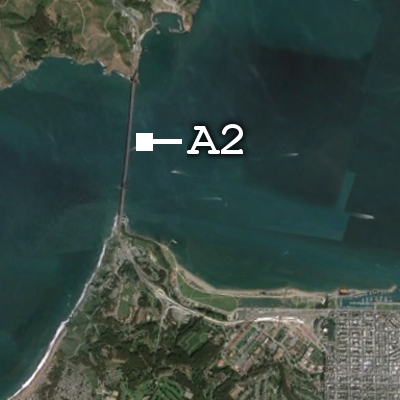
\includegraphics[width=\columnwidth]{Figures/ALOS2_SF_3Class/GoldenGateIm} 
\vspace{0.2cm}
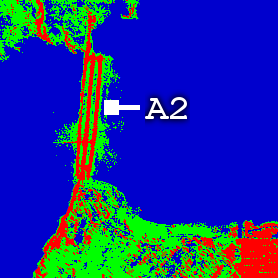
\includegraphics[width=\columnwidth]{Figures/ALOS2_SF_3Class/GoldenGate}
\caption{}
\label{fig:cla2_b}
\end{subfigure}
%\begin{subfigure}[t]{0.31\columnwidth}
%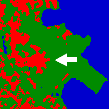
\includegraphics[width=\columnwidth]{Figures/RS2_SF_3Class/sfo_cl}
%\caption{Richmond}
%\end{subfigure}
\begin{subfigure}[t]{0.19\textwidth}
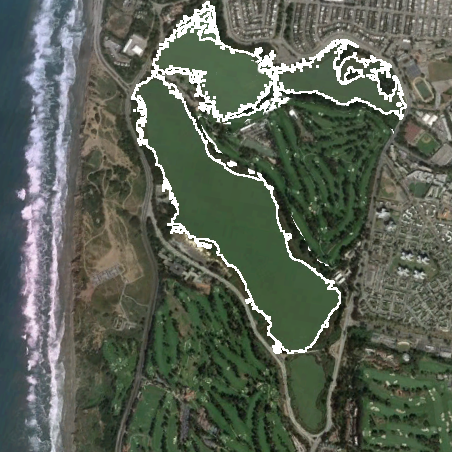
\includegraphics[width=\columnwidth]{Figures/ALOS2_SF_3Class/Lake} 
\vspace{0.2cm}
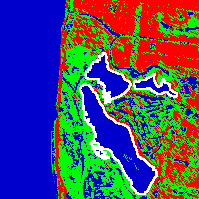
\includegraphics[width=\columnwidth]{Figures/ALOS2_SF_3Class/Lake_cl}
\caption{}
\label{fig:cla2_c}
\end{subfigure}
%\begin{subfigure}[t]{0.31\columnwidth}
%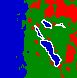
\includegraphics[width=\columnwidth]{Figures/RS2_SF_3Class/merced_cl}
%\caption{San And. Lake}
%\end{subfigure}
%\begin{subfigure}[t]{0.16\textwidth}
%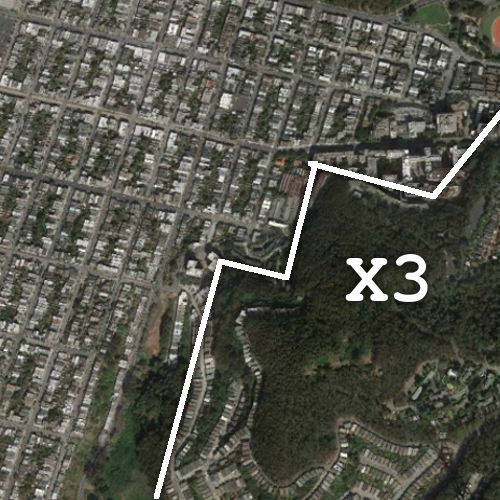
\includegraphics[width=\columnwidth]{Figures/ALOS2_SF_3Class/McLarenIm}
%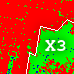
\includegraphics[width=\columnwidth]{Figures/ALOS2_SF_3Class/McLaren}
%\caption{UCSF}
%\label{fig:cl_d}
%\end{subfigure}
%\begin{subfigure}[t]{0.31\columnwidth}
%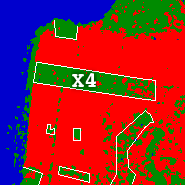
\includegraphics[width=\columnwidth]{Figures/RS2_SF_3Class/BotGard_cl}
%\caption{Sunset Blvd.}
%\end{subfigure}
\begin{subfigure}[t]{0.19\textwidth}
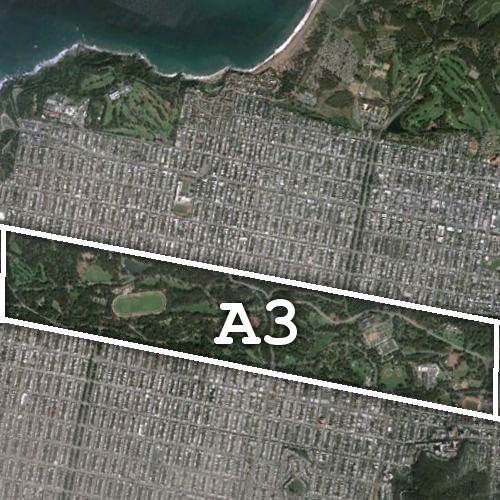
\includegraphics[width=\columnwidth]{Figures/ALOS2_SF_3Class/SunsetIm} 
\vspace{0.2cm}
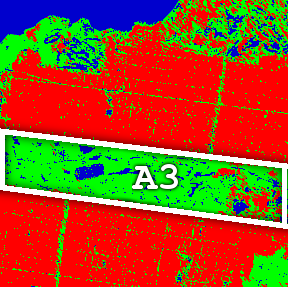
\includegraphics[width=\columnwidth]{Figures/ALOS2_SF_3Class/Sunset}
\caption{}
\label{fig:cla2_e}
\end{subfigure}
%\begin{subfigure}[t]{0.31\columnwidth}
%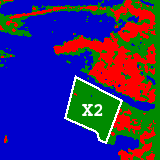
\includegraphics[width=\columnwidth]{Figures/RS2_SF_3Class/OaklandPort_cl}
%\caption{Port Oakland}
%\end{subfigure}
\begin{subfigure}[t]{0.19\textwidth}
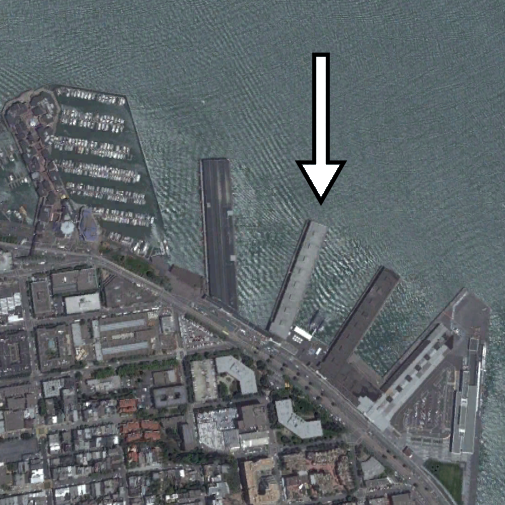
\includegraphics[width=\columnwidth]{Figures/ALOS2_SF_3Class/JettyIm} 
\vspace{0.2cm}
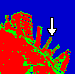
\includegraphics[width=\columnwidth]{Figures/ALOS2_SF_3Class/Jetty}
\caption{}
\label{fig:cla2_f}
\end{subfigure} %
%\begin{subfigure}[t]{0.31\columnwidth}
%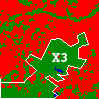
\includegraphics[width=\columnwidth]{Figures/RS2_SF_3Class/jmpark_cl}
%\caption{Port Oakland}
%\end{subfigure} 
\caption{Crops of the classified map shown alongside corresponding aerial imagery courtesy ESRI/Bing Maps.}
\label{fig:cl_crop_alos2}
\end{figure}




\subsubsection{Analysis of Classification Performance}
\label{sec:EXPT2}
%The ALOS-2 dataset collected over San Francisco, CA is classified using the described methodology. This radar operates in the L-band ($\lambda = 24 $cm). 


%These areas however return a much stronger echo in the C-band data set, as the surface perturbations are comparable to the radar wavelength in that case causing the return to be non-specular~\cite{lee2009polarimetric}. 



The Pauli composite image generated from the dataset is shown in Figure~\ref{fig:train1alos2} along with the training areas superimposed on it. They are derived from the interpretation of aerial imagery (ESRI/Bing Maps), topographical maps (USGS) and the Pauli composite and are marked with red polygons for urban areas, green for forest/vegetation areas, and blue for water. The pixels enclosed in these polygons form the ground truth. The proportion of ground-truth pixels in each class is approximately the same, and in total, they constitute less than $\sim10\%$ of the total pixels in the image. These are randomly divided into three groups: training, test and validation. Pixels in the training set are used in the training of the network. At regular intervals within the training iterations, the process is halted and the test pixels are used to evaluate the accuracy of the network. The difference between the training and test accuracy is used to ensure that the training phase is progressing without over-fitting or memorization. To quantify the final performance of the classifier, validation pixels are employed. The confusion matrix is and is presented in Table~\ref{tab:alos2tab}.

%From these ground-truth pixels, $\frac{1}{}$ the pixels are randomly selected as training pixels, and the rest are reserved for test. A testing phase is run every 1000 iterations which measures the accuracy of prediction over this labeled set. 












\begin{table}[tbp]
	\caption{Confusion matrix and accuracy statistics for ALOS-2 San Francisco, CA dataset using the proposed supervised classification scheme incorporating textural information}
	\label{tab:alos2tab}
	\begin{tabularx}{\columnwidth}{X|XXX|X}
		& Urban & Water  & Forest & Prod. Acc. \\ \hline
		Urban & \bf{84.20} & 0 & 4.39 & 95.45  \\
		Water & 1.3 & \bf{96.86} & 3.41 & 96.00 \\
		Forest & 14.5 & 3.14 & \bf{92.20} & 84.41\\ \hline 
		User Acc. & 84.85 & 96.97 &   92.93 & \\ \hline
		OA &  91.63 \% & & &  \\
		Kappa & 0.85 & & &  \\
	\end{tabularx}
\end{table}


% Alos-2 images'
\begin{figure}[tbp]
\centering
		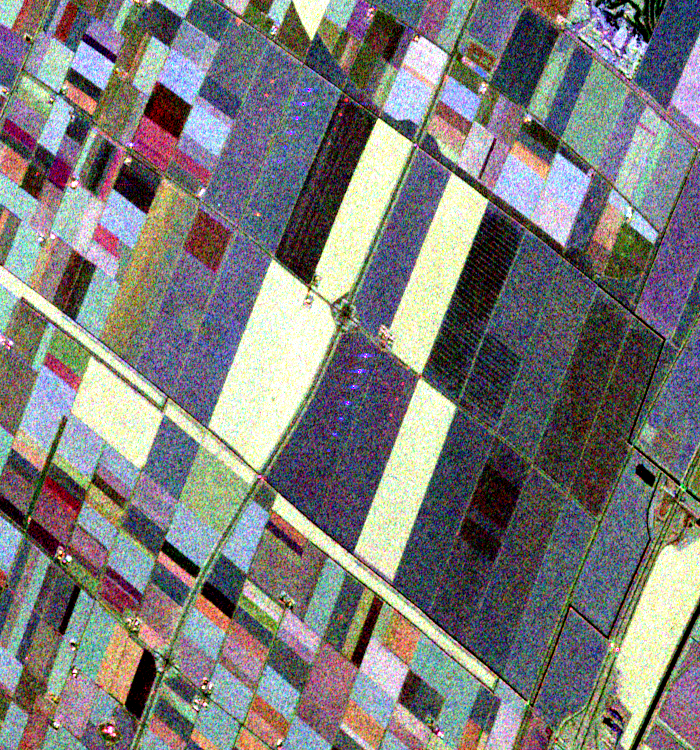
\includegraphics[width=0.5\columnwidth]{Figures/ALOS2_SF_3Class/Train}
		\caption{Pauli RGB image constructed from the ALOS-2 dataset collected over San Francisco, USA is shown with the ground-truth areas. The urban class is enclosed in red, the forest/vegetation in green and water in blue polygons.}
		\label{fig:train1alos2}
\end{figure}

\begin{figure}[tbp]
\centering
		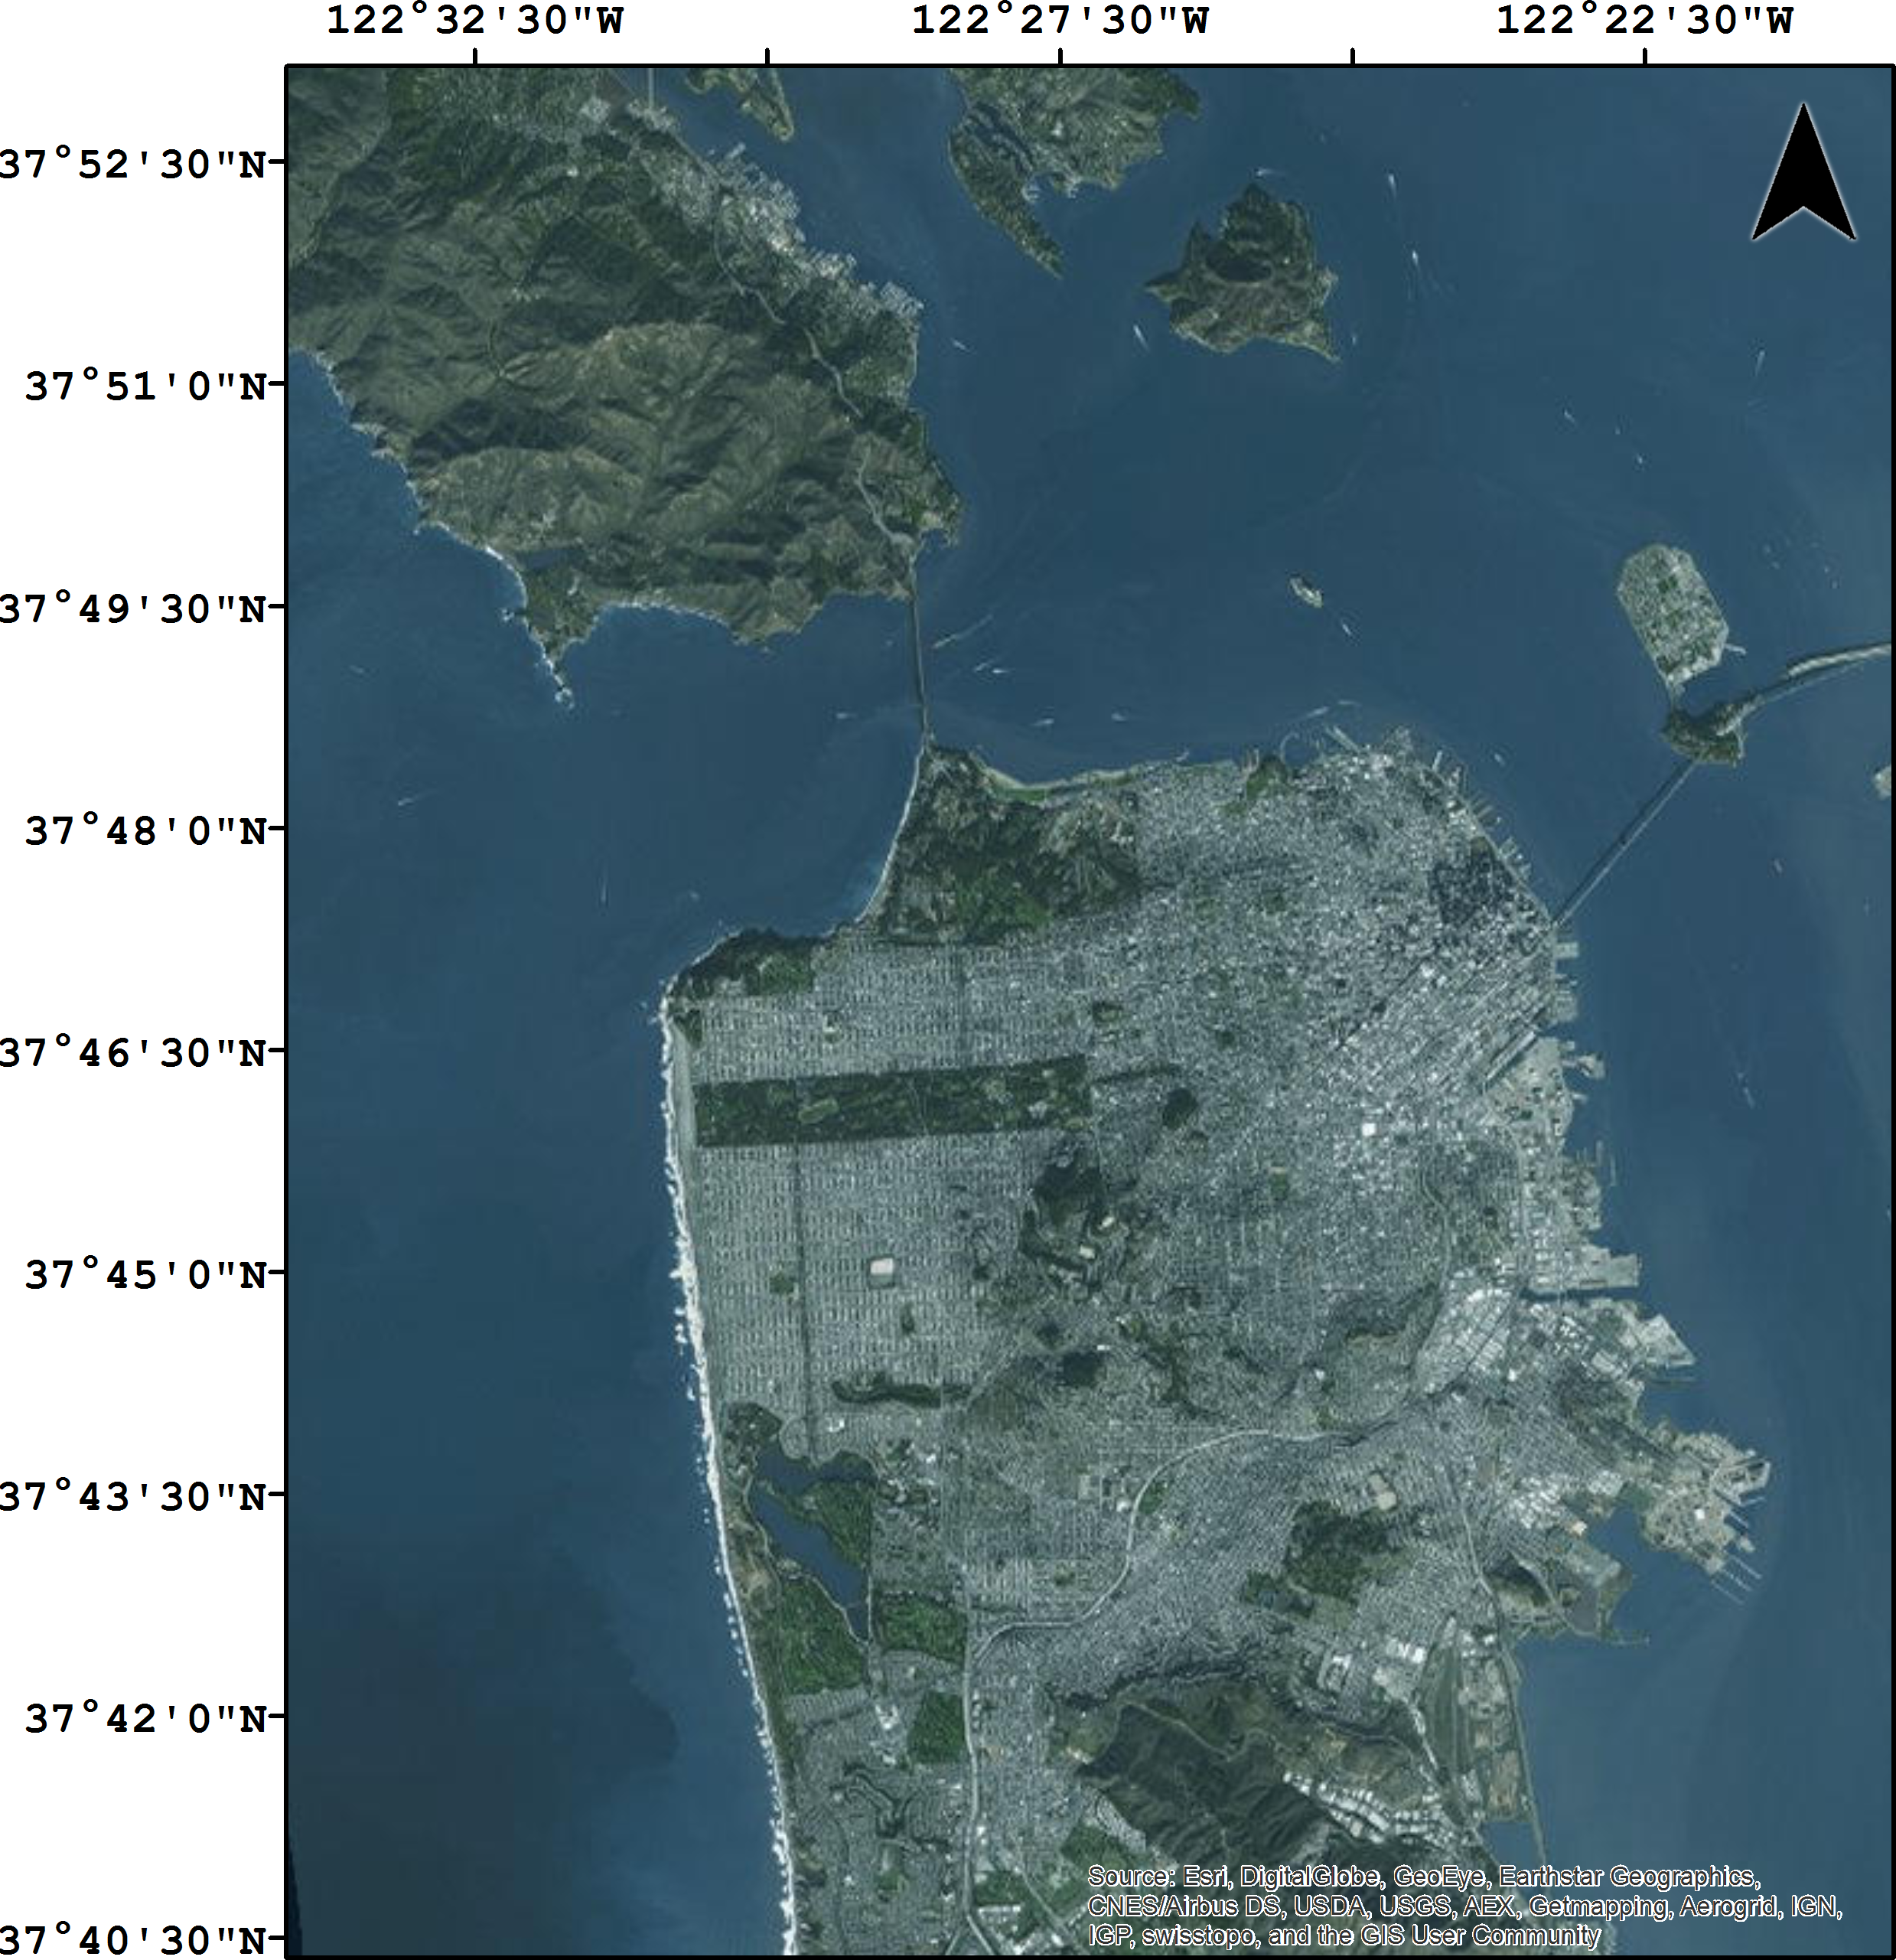
\includegraphics[width=0.5\columnwidth]{Figures/SF}
		\caption{Aerial imagery collected over San Francisco, USA depicting the extent covered by the ALOS-2 dataset courtesy of ESRI/Bing Maps.}
		\label{fig:OpticalAlos2}
\end{figure}

\begin{figure}[tbp]
	
	\begin{subfigure}[t]{0.19\textwidth}
		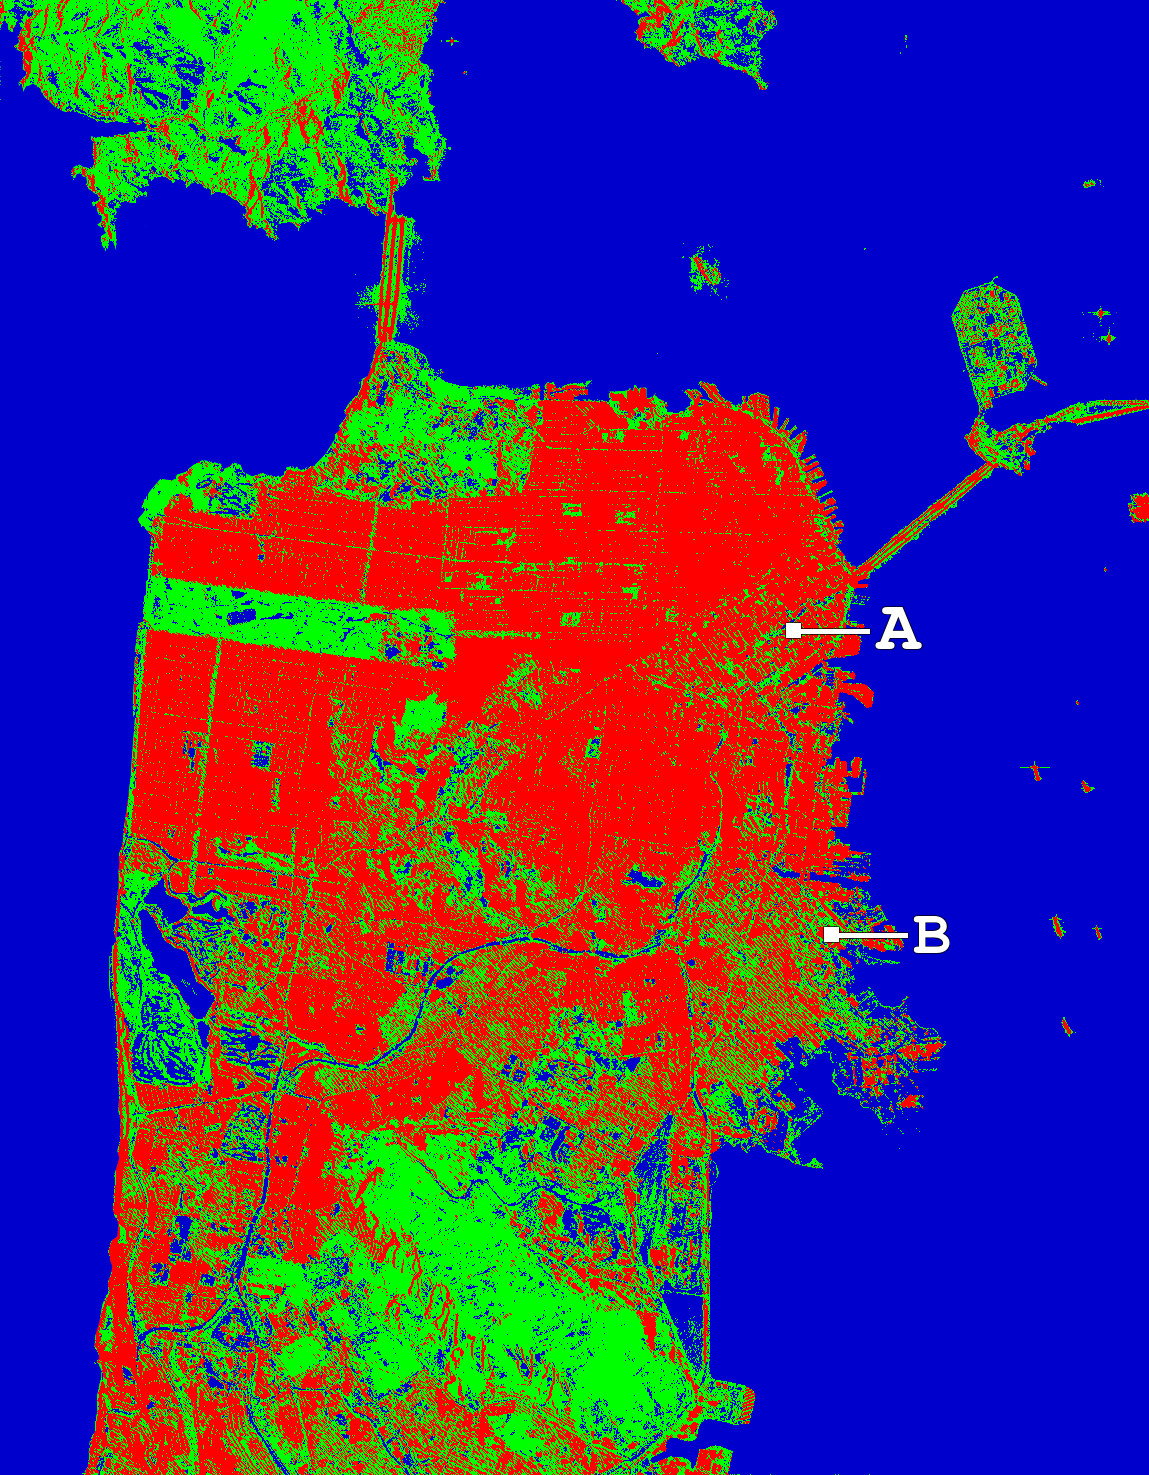
\includegraphics[trim={150px 80px 40px 50px},clip,width=\columnwidth]{Figures/ALOS2_SF_3Class/OP_300} 
		\caption{Proposed}
		\label{fig:proposed_al2}
	\end{subfigure}
	\begin{subfigure}[t]{0.19\textwidth}
		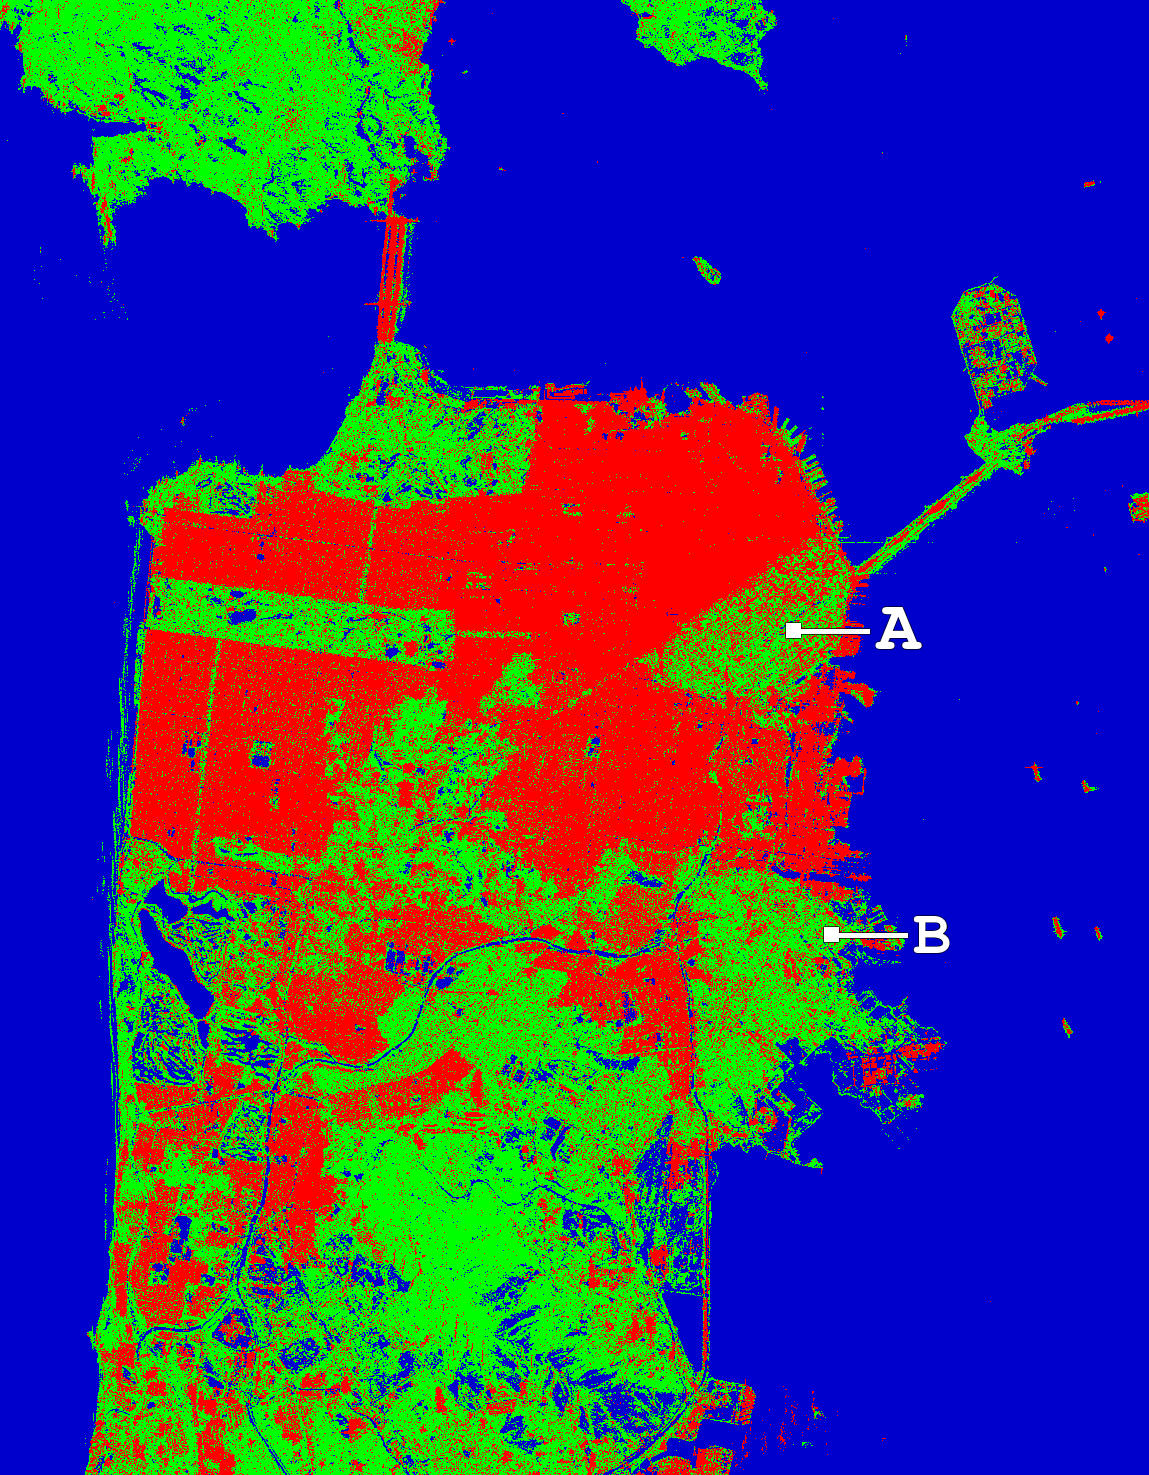
\includegraphics[trim={150px 80px 40px 50px},clip,width=\columnwidth]{Figures/ALOS2_SF_3Class/svm_classification_file_2016_04_07_12_23_47_rbf} 
		\caption{SVM RBF}
		\label{fig:al2_svm_rbf}
	\end{subfigure}
	\begin{subfigure}[t]{0.19\textwidth}
		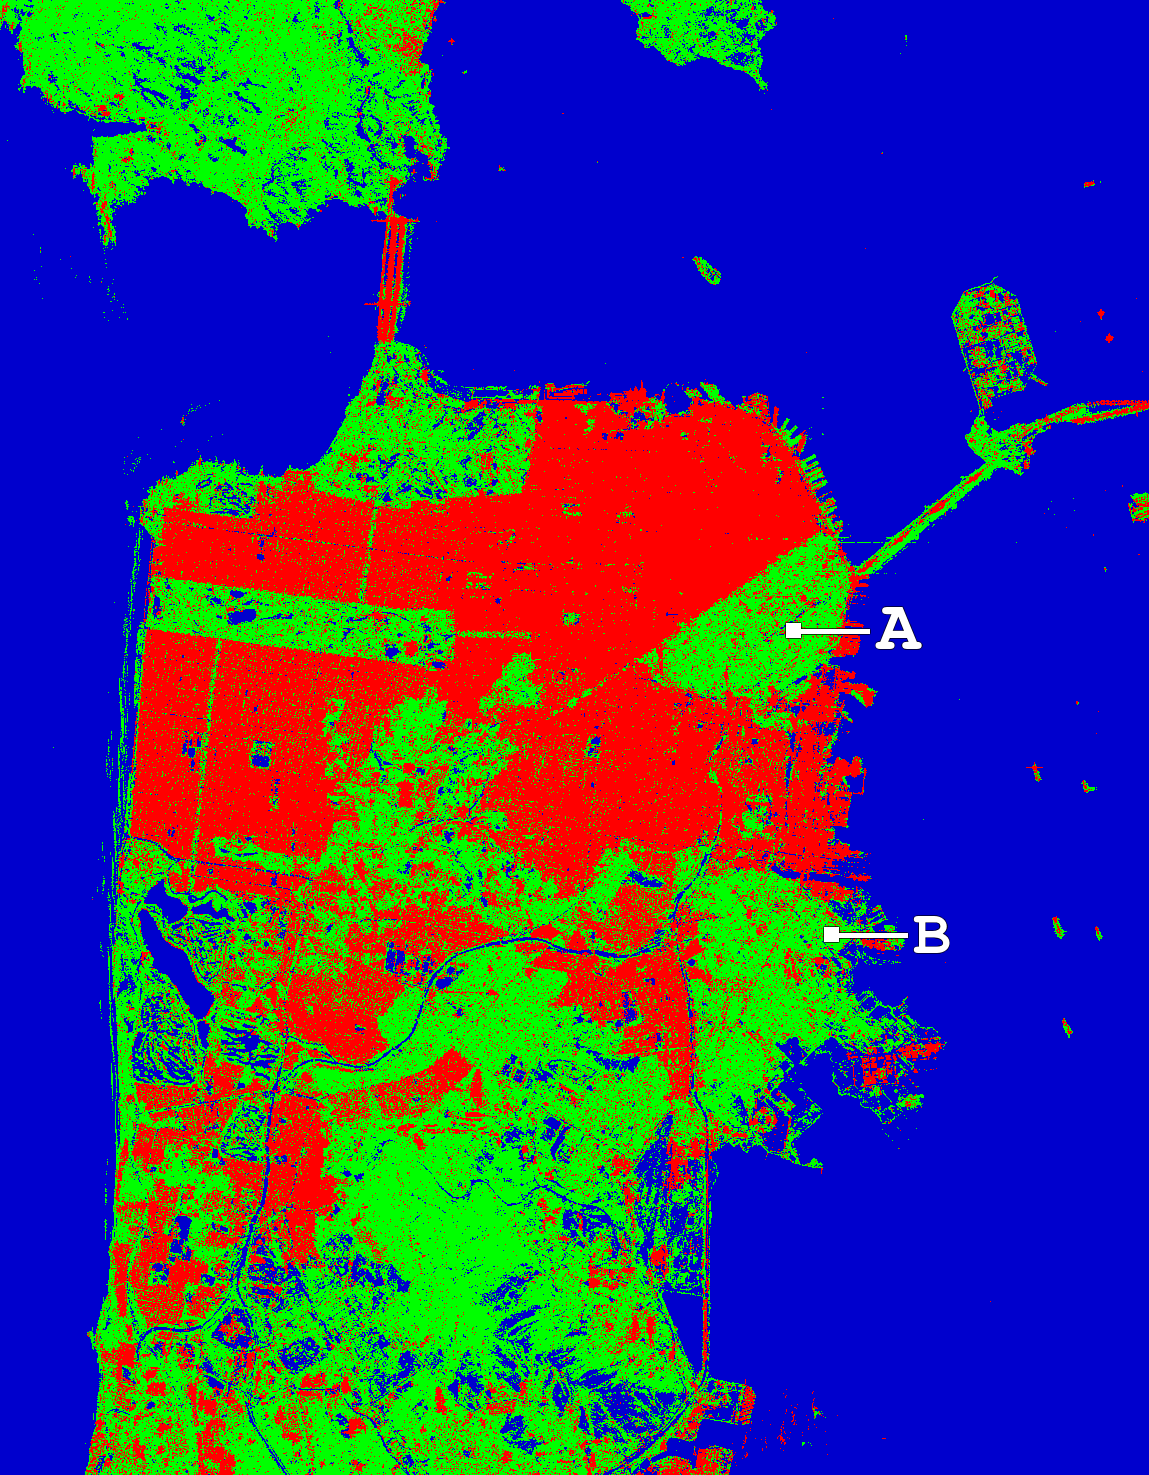
\includegraphics[trim={150px 80px 40px 50px},clip,width=\columnwidth]{Figures/ALOS2_SF_3Class/svm_classification_file_2016_04_07_12_20_26_lin} 
		\caption{SVM Polynomial}
		\label{fig:al2_svm_poly}
	\end{subfigure}
	\begin{subfigure}[t]{0.19\textwidth}
		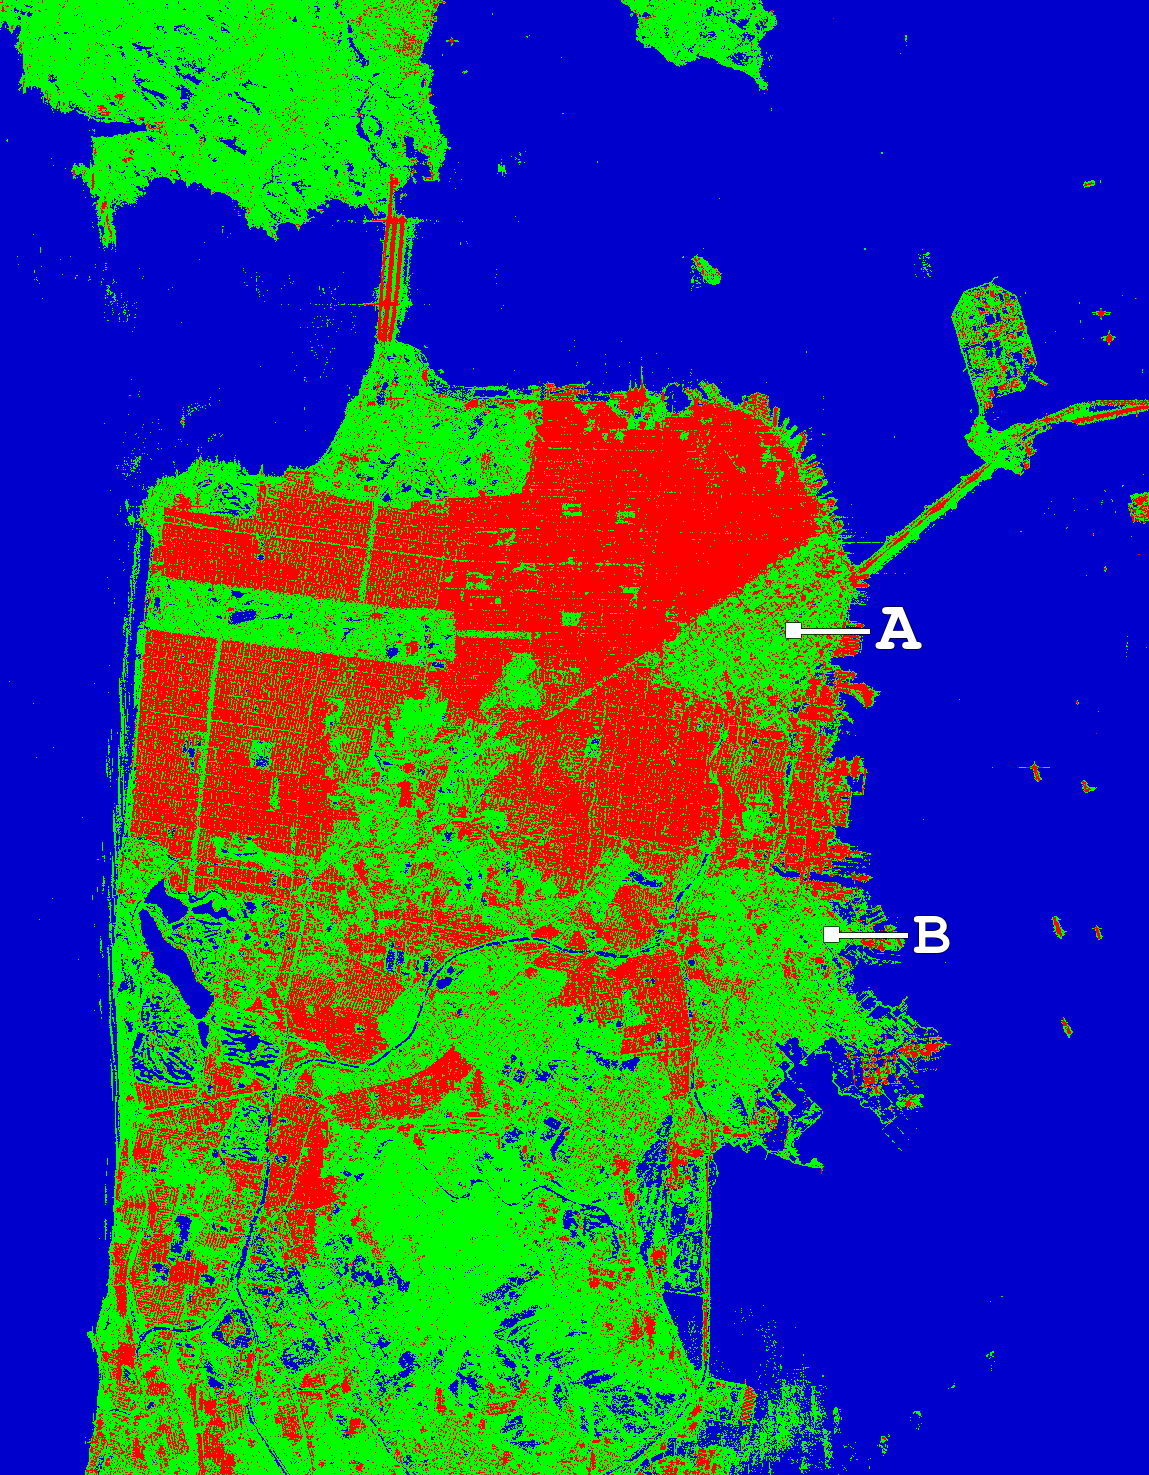
\includegraphics[trim={150px 80px 40px 50px},clip,width=\columnwidth]{Figures/ALOS2_SF_3Class/wishart_supervised_class_1x1_poc} 
		\caption{Wishart with POC}
		\label{fig:al2_wish_1_poc}
	\end{subfigure}
	\begin{subfigure}[t]{0.19\textwidth}
		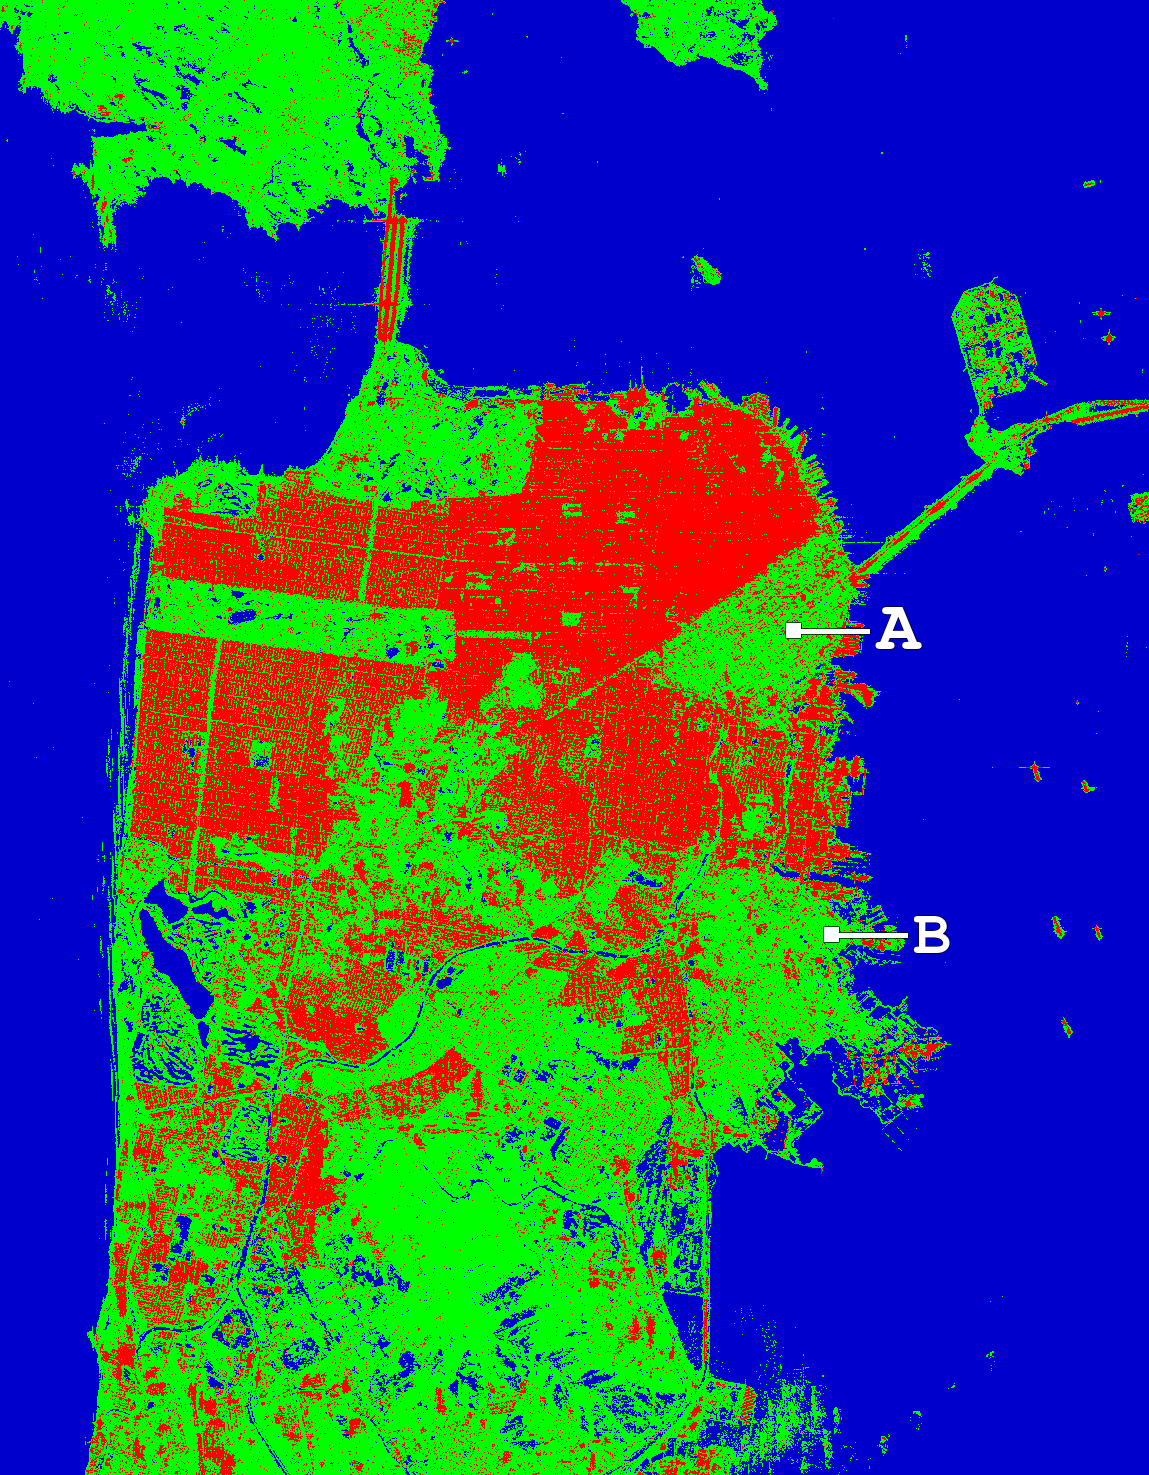
\includegraphics[trim={150px 80px 40px 50px},clip,width=\columnwidth]{Figures/ALOS2_SF_3Class/wishart_supervised_class_1x1} 
		\caption{Wishart}
		\label{fig:al2_wish_1}
	\end{subfigure}
	\caption{Comparison of common classification techniques with the proposed method.}
	\label{fig:comparison_al2}
\end{figure}

The dataset is classified with an overall accuracy of $91.63\%$ and a Kappa coefficient of 0.85. Urban areas are classified with an accuracy of $84.2\%$. The urban class is mostly confused with the forest class. This is primarily due to the fact that both, urban areas rotated with respect to the radar line of sight and vegetation have higher cross-polarized return. Certain small, smooth vegetated areas like parks. have been misclassified as the water class, contributing to the error of $3.14\%$ due to the low backscattered power as  previously highlighted. 

The resultant  map is presented in~Figure~\ref{fig:compwal2}. Reference aerial photographs are given in Figure~\ref{fig:OpticalAlos2}. We can see a close correspondence between the areas that appear to be urban in the optical aerial images and the  classification result. %This is unlike the Pauli composite image where the urban a[]reas behave like vegetation.
Detail subsets from selected areas of the classification output along with the corresponding aerial imagery, representing the ground truth, are shown in Figure~\ref{fig:cl_crop_alos2}. This demonstrates the performance of the proposed algorithm on the considered dataset. The resolution of this imagery is $\sim0.3m$ and is significantly higher than that of the classified map. However, reasonable correspondence can be seen between the two. 



%Detail crops of the classified output from the proposed method is shown in Figure~\ref{fig:cl_crop_alos2} along side aerial imagery of the same area. 
%The resolution of the the aerial is about $\sim$0.3m whichis more  comparable to the 6m effective resolution of ALOS-2 than the RadarSAT-2 dataset. 


The subset shown in Figure~\ref{fig:cla2_a} represents a dense urban area that is oriented at an angle $\sim-20^\circ$ from the radar line of sight, marked as Area `A1' in the image. Due to this large orientation, this region is often misclassified~\cite{lee11_5491157}, however it is classified correctly using the proposed method. %The proposed method involves the synthetic rotation of the data which is then given as input to the first auto-encoder stage. This causes a generalized target representation to be learned by the structure. We extract features from the auto-encoder which is representative of the response from the target and its possible orientations. In the third stage the MLP classifier is able to leverage this additional information to successfully classify this area. The auto-encoder stage is thus able to incorporate the additional information from the  synthetic rotated datasets into the classification scheme. 
% ~\cite{zhang2011extraction} bridge 
The subset shown in Figure~\ref{fig:cla2_b} shows the Golden Gate bridge, marked as `A2' and some surrounding areas. Apart from the return from the bridge itself,   multi-path returns from reflections from the bridge and the water surface can also be seen. The radar echoes from the vicinity of the bridge are quite strong and have a high value of $\gamma^0$. This causes the third stage of the classifier, which takes $\gamma^0$ as an input, to classify this pixels immediately under the bridge as forest. 
Figure~\ref{fig:cla2_c} shows a lake surrounded by urban and vegetated areas. This is marked with a white outline on the aerial images and classification maps.  It can be seen that the lake  is well discriminated from other classes. As discussed earlier, the smooth vegetated surfaces near the lake are misclassified as water due to near specular reflection at L-band frequencies and low incidence angles. 

The area marked as `A3' in the subset shown in Figure~\ref{fig:cla2_e} consists of a park between two regions of high density urban areas. It can be seen that the area of vegetation is well identified. The high resolution of ALOS-2 allows the faithful classification of small features in this park as well.  To further exploit high resolution datasets like ALOS-2 for classification of fine details, it is possible to avoid filtering operations in the SAR pre-processing step. Since, the proposed technique is pixel based, it does not cause a degradation in resolution.  
% Since the proposed technique does not require a window based processing, it is able to take advantage of the high spatial resolution of the ALOS-2 dataset. 
Subset shown in Figure~\ref{fig:cla2_f} is of a jetty. The white arrow marks a pier structure which has interleaving perpendicular cylindrical masts. This shows a high double bounce return which does not reduce with rotation of the target about the radar line of sight. This enables the classifier to correctly identify this structure. %The floor of the pier is made of wood and asphalt and is classified into the non-urban class. 

% % % % % % % % % % % % % % % % % % % % % % % % % % % % % % % %
%The methodology is also applied to a RADARSAT-2 C-band dataset and similar results are obtained (Figure~\ref{fig:RSAT}). The resolution of the dataset is slightly lower, thus it is not possible to discern individual building and road structure as seen in the ALOS-2 results, however the classification output is satisfactory and the developed technique is not limited by sensing frequency. 






% % RSAT
%\begin{figure}[!htb]
%		\centering
%	\begin{subfigure}[t]{0.45\columnwidth}
%	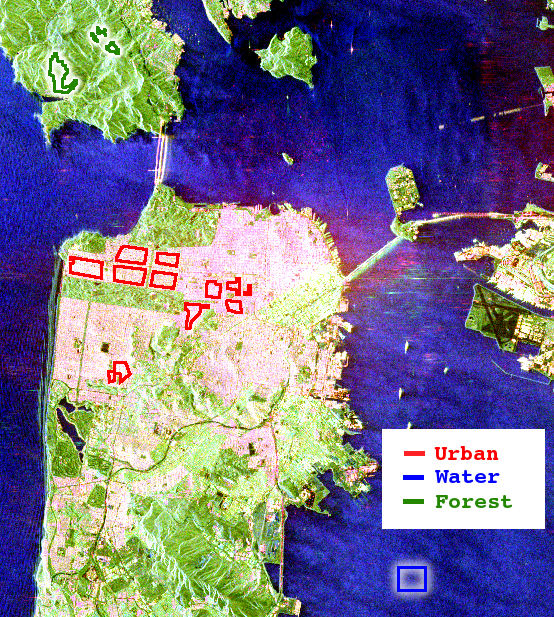
\includegraphics[width=\columnwidth]{Figures/RS2_SF_3Class/TrainingAreasCrop.png}
%		\label{fig:output}
%		\caption{Training areas}
%	\end{subfigure}
%	~
%	\begin{subfigure}[t]{0.45\columnwidth}
%	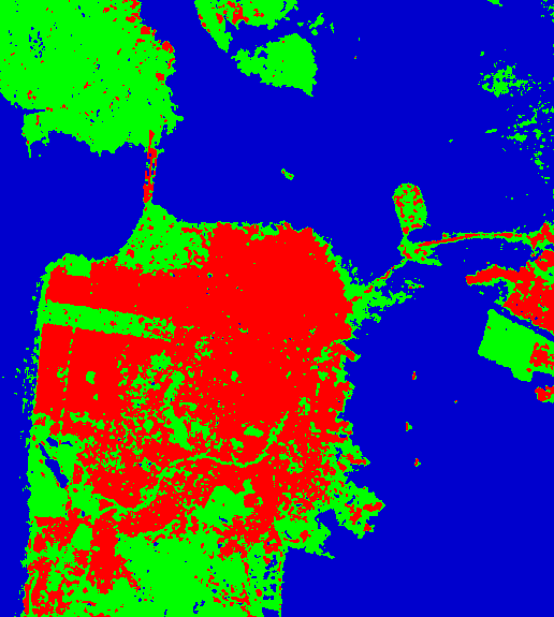
\includegraphics[width=\columnwidth]{Figures/RS2_SF_3Class/OUTPUT_3x3_CROP.png} 
%	\label{fig:output1}
%	\caption{Classification Map}
%	\end{subfigure}
%%	~	
%	\begin{subfigure}[b]{\columnwidth}
%	\centering
%	\begin{tabular}{clclcl}
%				
\includegraphics[width=0.015\columnwidth]{Figures/RS2_SF_3Class/Blue.png} & Water &		
\includegraphics[width=0.015\columnwidth]{Figures/RS2_SF_3Class/Green.png} & Forest &  	
\includegraphics[width=0.015\columnwidth]{Figures/RS2_SF_3Class/Red.png} &  Urban 
%	\end{tabular}
%	\end{subfigure}
%
%\caption{Classified map of San Francisco derived from an RADARSAT-2 full polarimeteric C-Band dataset acquired on 9 April 2009 if FQ-2 mode. }
%		\label{fig:RSAT}
%\end{figure}
%



%%%%%%%%%%%%%%%%%%%%%%%%%%%%%%%%%%%%%%%%%%%%%%%%%%%%%%%
\subsubsection{Analysis of the Learned Representation}
\label{sec:EXPT3}
%Analysis of the Auto-Encoder Action

\begin{figure}[tbp]
	\centering
	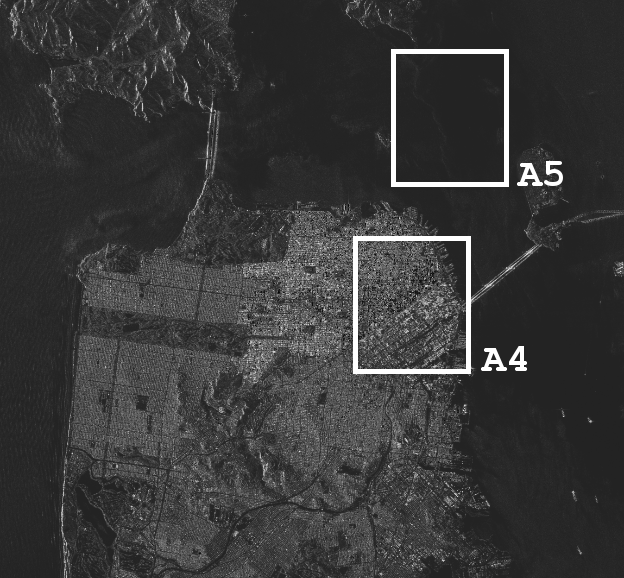
\includegraphics[width=0.85\columnwidth]{Figures/Wr_decode3_11_g}
	\\
	
\includegraphics[width = 0.3\columnwidth]{Figures/Rotation_FS/GRAY}
	\caption{Extracted feature map for one of the internal nodes in the representation layer from the trained AE.}
	\label{fig:wr}
\end{figure}

To understand the information encoded in the representational layer of the AE, the response of one of the nodes it is extracted and shown in  Figure~\ref{fig:wr} after the completion of the training phase. This is one of the many internal representations encoded by the network. Since the network is initialized randomly, the exact position of the internal node containing information and its encoding will change each time the network is trained. However, in general, it is observed that each internal node learns a different encoding of the data-set. 
The representation is sparse in nature with only small percentage of nodes containing useful information for classification. 
Area `A4' consists of urban areas both perpendicular to and oriented away from the radar line of sight. Although they appear distinct in the Pauli visualization (Figure~\ref{fig:train1alos2}), the trained network evokes a uniformly strong response from the area. Thus the AE is able to combine the information from the synthetically rotated urban target database to form an internal representation that is independent of the target orientation. This allows for the accurate classification of the urban areas. In contrast, homogeneous areas like Area `A5' have a lower response allowing them to be distinguished  in the final classification.  
	%- one of the many internal representations
	%- each representation learns a different encoding
	%- sparse repn with only some features having useful data
	%- we see that in area A - urban - irrespective of the orientation the network has a strong response 
	%- in contrast in area B lower response.
	%- this property of the NN allows it to classify



\subsubsection{Comparison with State of the Art Classifiers}
\label{sec:EXPT4}


\begin{table}[tbp]
\centering

\caption{Class-by-class test-area accuracy statistics for ALOS-2, San Francisco, CA dataset for the proposed technique, SVM with RBF kernel, the SVM with Polynomial kernel and the Wishart supervised classifiers. }
\label{tab:alos_comparison} 
\begin{tabularx}{\columnwidth}{X|XXXXX} 
 & Proposed & SVM-RBF  & SVM-Poly & Wishart + POC& Wishart  \\ \hline
Urban & 86.2 & 64.2 & 58.5 & 59.1 & 55.6 \\
Water & 98.1 & 96.4 & 96.3 & 92.1 & 92.1 \\
Forest & 86.1 & 84.2 & 83.6 & 83.2 & 82.8 \\ \hline
OA & 90.8  & 81.6 & 79.4 & 78.14 & 76.83  \\ 
\end{tabularx}
\end{table}

The proposed method is compared with other commonly used SAR classification techniques. The same training areas were used to train all classifiers.
%The ALOS-2 dataset collected over San Francisco has been classified using the proposed method, 
%the Wishart supervised classifier, and SVM classifiers with a polynomial and radial basis function (RBF) based kernel. 
%The same training areas were used to train all classifiers. 
%A crop of the results are presented in Figure~\ref{fig:comparison_al2}. The areas shown in the crop, marked `A' and `B', are highly urbanized as seen in the optical image collected over the area shown in~Figure~\ref{fig:OpticalAlos2}. However, it is only classified successfully the proposed method. The other  methods misclassify it as forest/vegetation because of its significant orientation. %The cross-polarized return from the area makes it difficult to discern this from actual areas of vegetation. However, due to the synthetic rotation the proposed scheme is able to account for this orientation information and more successfully classify the data, while maintaining high textural fidelity. 


The class-by-class accuracy is reported in Table~\ref{tab:alos_comparison} and the results are presented in Figure~\ref{fig:comparison_al2}. The SVM classifier was run with two kernels: a polynomial kernel (SVM-Poly) and a RBF kernel (SVM-RBF). The parameters of the RBF kernel were determined by the method described in~\cite{liu2011gaussian}. The polynomial kernel used has a degree of 4. The Wishart classifier was run both with Polarization Orientation Correction  (Wishart+POC) and without (Wishart). The proposed classifier has an urban area classification accuracy of 86.2\%. It outperforms the SVM-RBF, SVM-Poly Wishart+POC and Wishart classifier which have urban area accuracies of 64.2\%, 58.2\%, 59.1\% and 55.6\% respectively. The POC is able to improve the discernibility. However, targets that are oriented significantly with respect to the radar line of sight are still misclassified. 

The areas shown in the subset, marked `A' and `B', are highly urbanized as seen in the optical image collected over San Francisco (Figure~\ref{fig:OpticalAlos2}).
The cross-polarized return from area `A' makes it difficult to discern this from actual areas of vegetation. However, due to the synthetic rotation the proposed scheme is able to account for the orientation information and more successfully classify the region than the other methods, while maintaining high textural fidelity. 
%On qualitative examination of the classified images, we find that the proposed method has the best performance. 
%It is able to classify more regions of area `A' correctly, followed by the SVM-RBF classifier. 
The mean orientation angle of area `B' is almost perpendicular to that of area `A', and the region is characterized by large open spaces between man-made structures. The mixed nature of the pixels makes classification more difficult. As seen in Figure~\ref{fig:proposed_al2}, the proposed technique correctly classifies these structures while largely preserving the texture. The other methods erroneously classify most of this region with the RBF kernel SVM performing  better than the polynomial kernel SVM and Wishart supervised classifier. Wishart+POC performs slightly better than SVM with the polynomial kernel.

